%It should identify a question, and a data set that you'll use to answer the question. Justify why the problem is important, and why you think the data set will allow you to (begin to) answer the question.
%
%Stylistically, the proposal should be written as though it were a memo to your manager (at whatever kind of enterprise might care about this question: either government, nonprofit, or industry). You should justify why it's worthwhile to this enterprise for you to work on the project for a few months, and why you think you're likely to succeed.

\documentclass[a4paper]{article}
  \usepackage{amsmath} 
  \usepackage{amssymb} 
  \usepackage{indentfirst} 
  \usepackage{mathrsfs}
  \usepackage{verbatim}
  \usepackage{hyperref}
  \usepackage{bbm}
  \usepackage{url}
  \usepackage{graphicx,float,subfigure}
  \usepackage{geometry}
   \PassOptionsToPackage{hyphens}{url}

  \geometry{left=3cm,right=3cm,top=2cm,bottom=2cm}  
   
  \author{Nanqing Dong (nd367), Ziyi Chen (zc286)} 
  \title{ORIE 4741 mid-term project} 
  
  

\begin{document}
%\maketitle

\centerline
{\LARGE \textbf{ORIE 4741 mid-term report}}
\centerline
{\large Nanqing Dong (nd367), Ziyi Chen (zc286)}
~\\
\noindent
\textbf{\large Introduction\\}
\indent
%We aim at recommending customized hospitals and treatments for a certain inpatient to lower mortality risk. However, whether a inpatient will survive is uncertain in advance and we have to predict.
We aim at predicting whether an inpatient is likely to survive, which helps recommending customized hospitals and treatments for him (her) to lower mortality risk. Such a prediction can be formulated into a binary classification problem, in which we train the classfier using the Statewide Planning and Research Cooperative System (SPARCS) Hospital Inpatient Discharges dataset [1]. This dataset has the discharge records with 39 variables of 2544731 patients. Among these variables, the ``inpatient disposition" tells us whether an inpatient survived upon discharge. Detail of these variables is shown in Table 1.\\

\noindent
\textbf{\large Data Preprocessing\\}
\indent
At first, we deleted irrelevant variables by common sense and kept 16 predictors as well as the variable called ``inpatient disposition". Then, we transformed the ``inpatient disposition" into the target variable called ``die", indicating whether a patient passed away ( ``die=1") or not (``die=0").\\
\indent
Moreover, we delete the 100130 patients with missing values, including global missing value ``na", and those specific to variables like ``Ethnicity=Unknown", ``Gender=U", etc.\\

\noindent
\textbf{\large Preliminary observation on the relevancy of each predictor\\}
\indent
Since all the predictors are categorical, we measure the relevancy of a predictor $X_j$ by the variation of the death rate with each value $k$ of $X_j$. The death rate for $X_j=k$ is defined as the percentage of the dead inpatients in the inpatients whose $X_j=k$. For each variable, we roughly measure its relevancy by the standard deviation of these death rates, as shown in Table 1.\\
\indent
It can be seen from Table 1 that the standard deviation of death rate for the variable ``APR Risk of Mortality", the diagnosed disease and its severity are among the highest, and that of the inpatients' gender and admitted day of the week are among the lowest, which also makes sense. Fortunately, the hospital (``facility id") and treatment (``CCS Procedure Code", ``APR MDC Code") we concern have comparable standard deviation to the highest one.\\
%However, the APR Risk of Mortality is based on severity of illness and does not take into account some factors like hospital ( ``Facility id") and treatments (``CCS Procedure Code", ``APR MDC Code") [2], which also have high and comparable standard deviation to that of ``APR Risk of Mortality". Hence, we can still improve its predictive accuracy by adding these factors, and thus recommending hospitals and treatments. In addition, as to the standard deviation of death rate, the diagnosed disease and its severity is among the highest, whereas the inpatients' ethnicity, gender and admitted day of the week is among the lowest, which also makes sense.
\indent
To go further into the relevancy of each predictor, we plot barcharts of these death rates for ``APR MDC Code" and ``Admit Day of Week", in Figure 1. Figure 1 (a) shows a large variation of death rate with ``APR MDC Code" (category of diagnosed disease). Among the diseases, ``Infectious and Parasitic Diseases, Systemic or Unspecified Sites" (18) has the highest death rate, whereas ``Pregnancy, Childbirth and the Puerperium" (14) has the lowest death rate, which also fits common sense. Figure 1 (b) shows very slight effect of inpatient's admitted day on the death rate. As it approaches the weekend, the death rate increases and reach the peak during the weekend, and dramatically falls to the lowest on Monday. In fact, this is reasonable since most staffs tend to be more responsible on weekday than on weekend.\\ 

\noindent
\textbf{\large Feature selection by mutual information\\}
\indent
Feature selection is an important method to avoid overfitting. Since the target and predictors are all categorical, we adopt a simple feature selection method based on the mutual information (MI) between each predictor and the target variable, a commonly used measure of relevancy between the two [3]. We compare these MI's and list them in decreasing order in Table 1. As shown in Table 1, MI is significantly correlated with standard deviation of death rate. We select the 10 predictors with the highest MI's from ``APR Risk of Mortality" to ``Emergency Department Indicator". \\

\noindent
\textbf{\large Naive Bayes Classification\\}
\indent
After feature selection, we adopt Naive Bayes classifer [3], a simple but popular classification method for categorical predictors. \\
\indent
To test the performance, we randomly partition the dataset into training dataset with 80\% of the samples and test dataset with 20\% of the samples. To avoid overfitting, we train the classifier with various smoothing parameter $\lambda$ using 5-fold cross-validation on the training dataset. Since there is a significant imbalance between the positive group (52721 samples whose ``die=1") and negative group (2391880 samples whose ``die=0"), we adopt F1 score instead of the proportion of misclassification error as the measure of performance. Finally, we list the F1 score on the test dataset and the mean F1 score on the 5 validation sets in Table 2, for $\lambda \in \{0,0.1,1,2,3,5,10,100\}$ respectively.\\
\indent
It can be seen from Table 2 that all these F1 scores are all slightly more than 0.30, far from the full mark 1.0, thus it requires more work later to improve the performance. In addition, the F1 scores on both the validation data and the test data keep slightly increasing with $\lambda$, which means it is likely to get more accurate prediction with larger $\lambda$.\\

\noindent
\textbf{\large Future work\\}
\noindent
%During November, we plan to do some improvement work:
1. Delete highly correlated predictors. \\%For example, there are 3 variables denoting diagnosed disease using 3 different diagnosis methods, respectively. We will look at the correlations among these variables and see if we can delete 1 or 2 of them.\\
\noindent
2. Delete samples: Some predictors have over 200 values, whereas some values are not representative enough due to limited samples, which could be deleted.\\
\noindent
3. We will try various ways to deal with imbalance between the 2 classes, such as bootstrap.\\
\noindent
4. Try more classifiers, and then use cross validation to choose the best classifier. \\
\noindent
5. Use the best classifier to recommend customized hospitals and treatments for a specific new patient that have small predicted death rate.\\

\begin{figure}[H]
\begin{center}
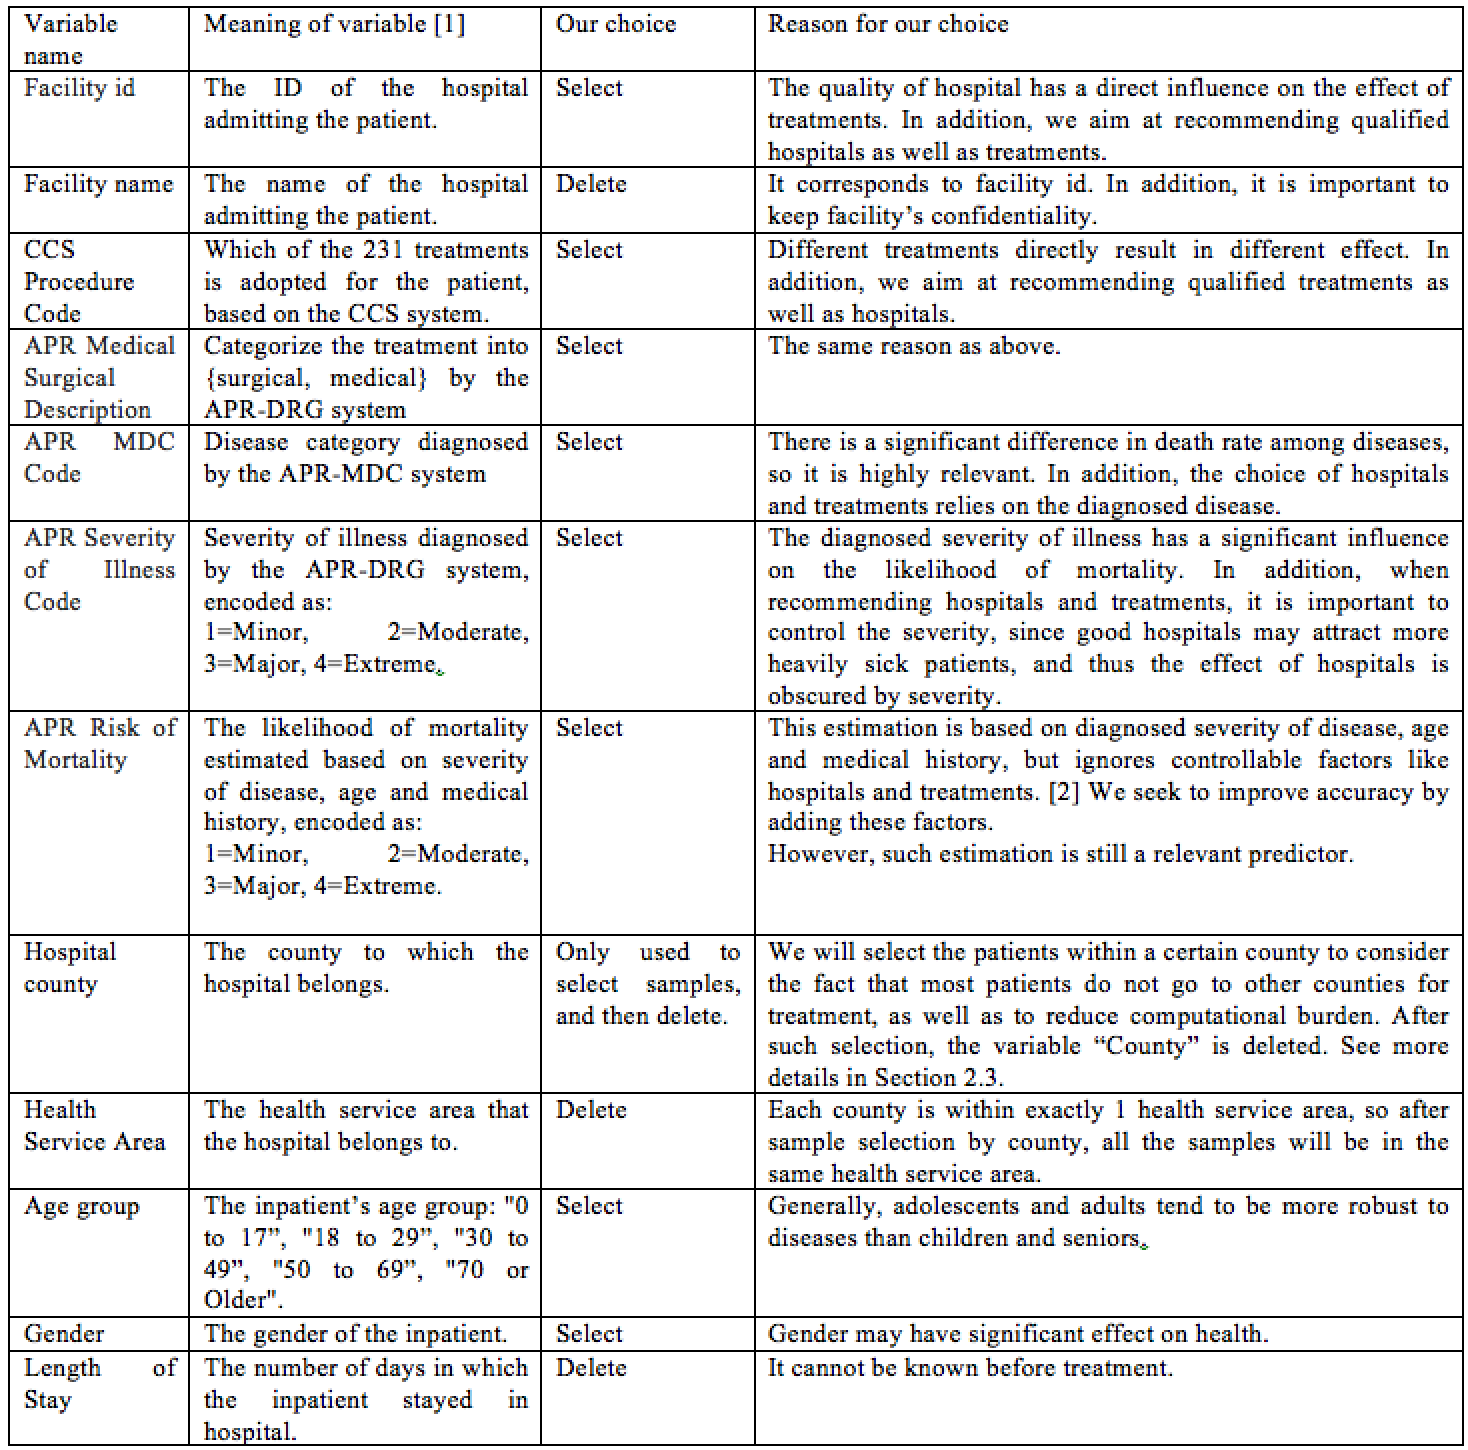
\includegraphics[width=5.0in]{table1_variable_information.png}
%\caption{Table 1: The 16 categorical predictors. \label{The 16 categorical predictors}}
\end{center}
\end{figure}
\centerline
{Table 1: The 16 categorical predictors [1]}

%\begin{figure}[H]
%\begin{center}
%\includegraphics[width=3.5in]{fig1_MDC.png}
%\caption{The death rate for each value of ``APR MDC Code (Diseases are encoded into 1\~25)" \label{Death Rate VS APR MDC Code}}
%\end{center}
%\end{figure}
%
%\begin{figure}[H]
%\begin{center}
%\includegraphics[width=3.5in]{fig2_admit_day.png}
%\caption{The death rate for each value of ``Admit Day of Week" \label{Death Rate VS Admit Day}}
%\end{center}
%\end{figure}

%\begin{figure}[H]
%\begin{minipage}[t]{0.5\linewidth}
%\centering
%\includegraphics[width=2.2in]{fig1_MDC.png}
%\caption{The death rate for each value of ``APR MDC Code}
%\label{fig:side:a}
%\end{minipage}%
%\begin{minipage}[t]{0.5\linewidth}
%\centering
%\includegraphics[width=2.2in]{fig2_admit_day.png}
%\caption{The death rate for each value of ``Admit Day of Week"}
%\label{fig:side:b}
%\end{minipage}
%\end{figure}

\begin{figure}[H]
  \centering
  \subfigure[``APR MDC Code"]{
    \label{fig:subfig:a} %% label for first subfigure
    \includegraphics[width=3in]{fig1_MDC.png}}
  \hspace{0in}
  \subfigure[``Admit Day of Week"]{
    \label{fig:subfig:b} %% label for second subfigure
    \includegraphics[width=3in]{fig2_admit_day.png}}
  \caption{The death rate for each value}
  \label{fig:subfig} %% label for entire figure
\end{figure}

%\begin{figure}[H]
%\centering
%\subfigure[Table 1: The 16 categorical predictors]{
%%    \label{fig:subfig:a} %% label for first subfigure
%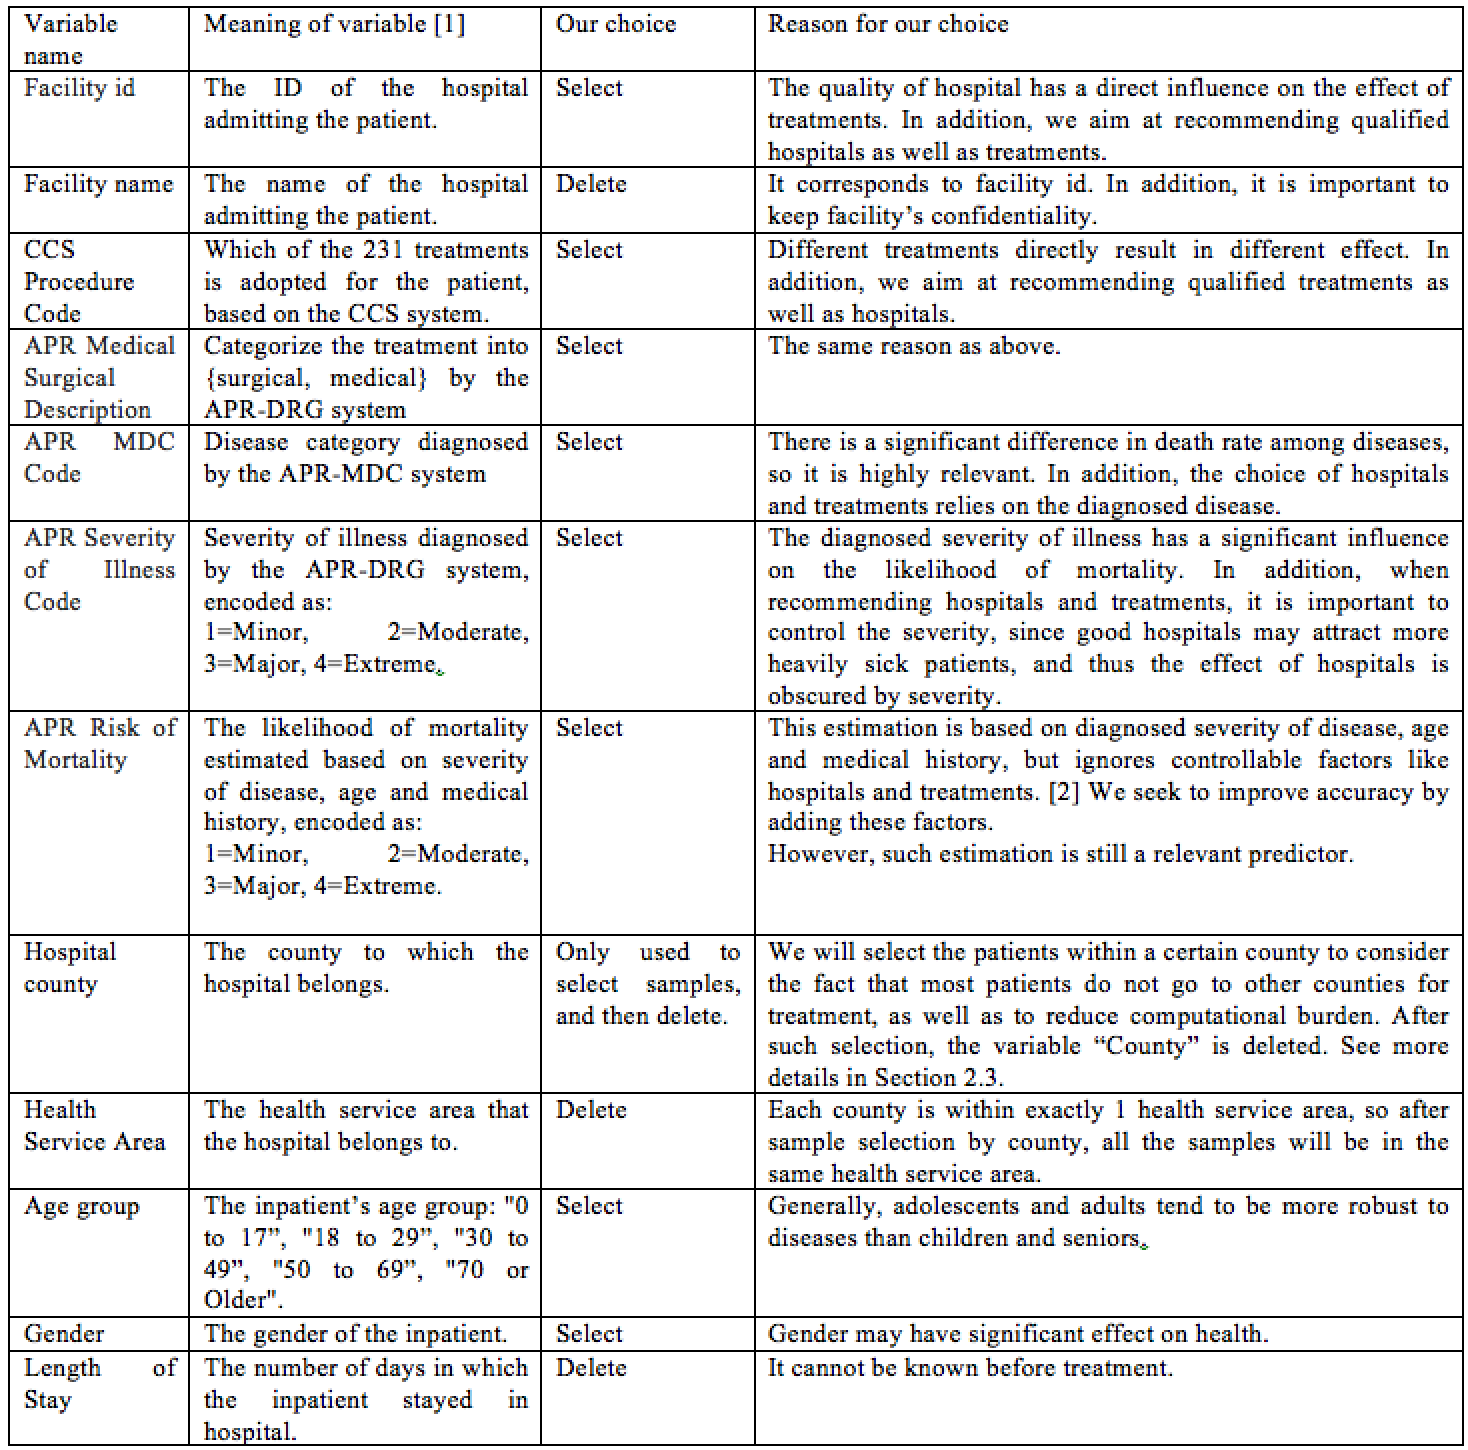
\includegraphics[width=2.2in]{table1_variable_information.png}}
%\hspace{0in}
%\subfigure[Table 2: The performance of naive Bayes classifier]{
%%    \label{fig:subfig:b} %% label for second subfigure
%\includegraphics[width=2.2in]{table2_F1_naive_Bayes.png}}
%%  \caption{}
%\label{fig:subfig} %% label for entire figure
%\end{figure}

\begin{center} 
    \begin{tabular}{|c|c|c|} 
       \hline 
      Smoothing & The mean F1 score on & The F1 score on\\ 
      parameter $\lambda$ & the 5 validation datasets & the test dataset\\ \hline    
      0 & 0.3048 & 0.3086 \\ \hline
      0.1 & 0.3051 & 0.3088 \\ \hline
      1 & 0.3054 & 0.3089 \\ \hline
      2 & 0.3057 & 0.3090 \\ \hline
      3 & 0.3060 & 0.3093 \\ \hline
      5 & 0.3064 & 0.3097 \\ \hline
      10 & 0.3067 & 0.3102 \\ \hline
      100 & 0.3071 & 0.3104 \\ \hline
    \end{tabular} 
\end{center}
 
\centerline
{Table 2: The performance of naive Bayes classifier}

~\\~\\
\noindent
\textbf{\large References\\}
\noindent
[1] Statewide Planning and Research Cooperative System (SPARCS) Hospital Inpatient Discharges dataset: \\
{\small {https://health.data.ny.gov/Health/Hospital-Inpatient-Discharges-\do SPARCS-De\\-Identified/u4ud-w55t}\\}

\noindent
[2] Baram, Daniel, et al. "Use of the All Patient Refined-Diagnosis Related Group (APR-DRG) risk of mortality score as a severity adjustor in the medical ICU." Clinical Medicine Insights. Circulatory, Respiratory and Pulmonary Medicine 2 (2008): 20.\\

\noindent
[3] Murphy, Kevin P. Machine learning: a probabilistic perspective. MIT press, 2012.

\end{document} 






